% !TeX root = ../main.tex
% %%%%%%%%%%%%%%%%%%%%%%%%%%%%%%%%%%%%%%%%%%%%%%%%%%%%%%%%%%%%%%%%%%%%%%%%%%%%%%
% Evaluation
\chapter{Evaluation}
\label{chap:evaluation}

This chapter introduces the evaluation process of the work. \autoref{sec:evaluationoverview} gives a broad overview of the whole process, and \autoref{sec:experiments} goes into more detail about each one of the experiments.


% ------------------------------------------------------------------------------
% Evaluation Overview
\section{Evaluation Overview}
\label{sec:evaluationoverview}

To evaluate the developed work, we decided to go through a list of already documented ROS bugs and identify three that happen at runtime. After that, we specified a robot's properties in the DSL that should be capable of detecting an error for said bugs while running the system.

ROBUST~\cite{robust} is a dataset that documents over two hundred bugs in multiple robots using ROS. After going through the dataset, three bugs were chosen:

\begin{itemize}
    \item Calculation Error Inverts Turning Direction~\footnote{\url{https://github.com/robust-rosin/robust/blob/master/kobuki/e964bbb/e964bbb.bug}} (\autoref{ssec:calculationerrorinvertsturningdirection}) - "Due to an error in velocity calculations, when Kobuki was issued a very low negative linear speed (very slow backwards movement), it would also inadvertently invert its turning direction. That is, if it was supposed to move backwards while turning left, it would move backwards and turn right instead."
    \item Robot Getting Stuck When Auto-docking~\footnote{\url{https://github.com/robust-rosin/robust/blob/master/kobuki/0416c81/0416c81.bug}} (\autoref{ssec:robotgettingstuckwhenautodocking}) - "The movement speeds were hard-coded for the auto-docking algorithm, and worked well for regular Kobuki and Turtlebot, but were too slow for heavier robots, causing them to get stuck."
    \item Unexpected Movement Due to Wrong Calculation~\footnote{\url{https://github.com/robust-rosin/robust/blob/master/kobuki/1c141a5/1c141a5.bug}} (\autoref{ssec:unexpectedmovementduetowrongcalculation}) - "Kobuki moves using differential drive. Originally, the command velocities (linear and angular) were provided as `short`, and were converted to `short` after each step, even though the calculations yielded floating point numbers. This lead to calculation errors in some special cases, where the robot was supposed to move forward but ended up moving backwards instead."
\end{itemize}

To replicate each bug, a \textit{demon} node is inserted into the system that interferes with the normal runtime flow and replicates the desired bug. \autoref{fig:normalflow} represents the natural flow of the systems whilst \autoref{fig:demonflow} shows the system flow when trying to replicate a bug with the help of the \textit{demon} node.

\begin{figure}
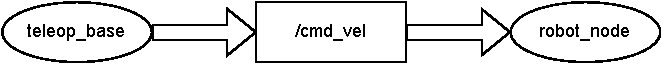
\includegraphics[width=\textwidth]{images/normal_flow.pdf}
\caption{Normal flow.} \label{fig:normalflow}
\end{figure}
    
\begin{figure}
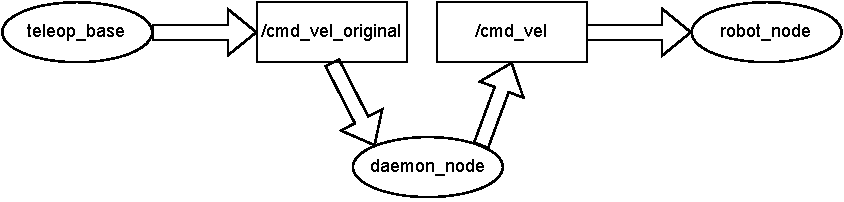
\includegraphics[width=\textwidth]{images/demon_flow.pdf}
\caption{Demon flow.} \label{fig:demonflow}
\end{figure}

When injecting a bug, all the data before addressed to the robots' \textit{/cmd\_vel} topic is remapped to a new topic called \textit{/cmd\_vel\_original}, the \textit{demon} node subscribes to this new topic and modifies the data before sending it to the robots' \textit{/cmd\_vel} topic so that the robot behaves like the expected bug. 

With this new system flow, it is possible to specify properties between the \textit{/cmd\_vel} topic which represents the robots' behavior, and the \textit{/cmd\_vel\_original} topic, which represents the actual command given to the robot.


% ------------------------------------------------------------------------------
% Experiments
\section{Experiments}
\label{sec:experiments}

This section goes through the property specification and runtime monitoring for the three mentioned selected bugs. Calculation Error Inverts Turning Direction (\autoref{sec:background}), Robot Getting Stuck When Auto-docking(\autoref{sec:background}), and Unexpected Movement Due to Wrong Calculation (\autoref{sec:background}).


% ------------------------------------------------------------------------------
% Calculation Error Inverts Turning Direction
\subsection{Calculation Error Inverts Turning Direction}
\label{ssec:calculationerrorinvertsturningdirection}

DSL property specification:

\texttt{decl angular\_vel\_robot\_perception cmd\_vel\_original Twist.angular.z}

\textit{T.}

\texttt{after turtlebot3.velocity.angular.z < 0, never angular\_vel\_robot\_perception > 0}

\textit{T.}

\textit{Demon} node code and behavior:

\begin{lstlisting}[language=python]
    class Direction_invert_error:

        def __init__(self):
            print("simulating direction_invert_error_behavior...")
            self.cmd_vel_pub = rospy.Publisher("cmd_vel", Twist, queue_size=1)
            self.twist = Twist()
            self.direction_invert_error()

        def get_vel(self):
            return rospy.wait_for_message("cmd_vel_original", Twist)

        def direction_invert_error(self):
            while not rospy.is_shutdown():
                vel = self.get_vel()
                self.twist = vel
                if abs(vel.linear.x) < 0.012:
                    self.twist.angular.z = -vel.angular.z
                self.cmd_vel_pub.publish(self.twist)
\end{lstlisting}

\textit{T.}


*explain what i do with teleop?*

*show output*


% ------------------------------------------------------------------------------
% Calculation Error Inverts Turning Direction
\subsection{Robot Getting Stuck When Auto-docking}
\label{ssec:robotgettingstuckwhenautodocking}

DSL property specification:

\texttt{decl vel\_robot\_perception cmd\_vel\_original Twist.linear.x}

\textit{T.}

\texttt{after vel\_robot\_perception > 0, never turtlebot3.velocity =={0.005} 0}

\textit{T.}

\textit{Demon} node code and behavior:

\begin{lstlisting}[language=python]
    class Auto_docking_error:

        def __init__(self):
            print("simulating auto_docking_error_behavior...")
            self.cmd_vel_pub = rospy.Publisher("cmd_vel", Twist, queue_size=1)
            self.twist = Twist()
            self.auto_docking_error()

        def get_vel(self):
            return rospy.wait_for_message("cmd_vel_original", Twist)

        def auto_docking_error(self):
            while not rospy.is_shutdown():
                vel = self.get_vel()
                self.twist = vel
                if abs(vel.linear.x) < 0.015:
                    self.twist.linear.x = 0.0
                self.cmd_vel_pub.publish(self.twist)
\end{lstlisting}

\textit{T.}


*explain what i do with teleop?*

*show output*


% ------------------------------------------------------------------------------
% Calculation Error Inverts Turning Direction
\subsection{Unexpected Movement Due to Wrong Calculation}
\label{ssec:unexpectedmovementduetowrongcalculation}

DSL property specification:

\texttt{decl vel\_robot\_perception cmd\_vel\_original Twist.linear.x}

\textit{T.}

\texttt{after turtlebot3.velocity.linear.x < 0, never vel\_robot\_perception > 0}

\textit{T.}

\textit{Demon} node code and behavior:

\begin{lstlisting}[language=python]
    class Backwards_movement_error:

        def __init__(self):
            print("simulating backwards_movement_error_behavior...")
            self.cmd_vel_pub = rospy.Publisher("cmd_vel", Twist, queue_size=1)
            self.twist = Twist()
            self.backwards_movement_error()

        def get_vel(self):
            return rospy.wait_for_message("cmd_vel_original", Twist)

        def backwards_movement_error(self):
            while not rospy.is_shutdown():
                vel = self.get_vel()
                self.twist = vel
                if abs(vel.linear.x) > 0.03:
                    self.twist.linear.x = -vel.linear.x
                self.cmd_vel_pub.publish(self.twist)
\end{lstlisting}

\textit{T.}


*explain what i do with teleop?*

*show output*
